
\documentclass[xcolor={dvipsnames}]{beamer}
\usepackage{amsmath,amsfonts,amssymb,pxfonts,eulervm,xspace}
\usepackage{graphicx}
 \usepackage{multimedia}
\usepackage{media9}
\usepackage{minted}
\usepackage{mathtools}

\usepackage{animate}

\graphicspath{{./figures/}}
\usetheme{ccnycrest}


\begin{document}

\title{ CS102: Functions }
\author{Hannah Aizenman}
\date{haizenm00@ccny.cuny.edu}


\begin{frame}
	\titlepage
\end{frame}

\begin{frame}[plain]
		\begin{figure}
	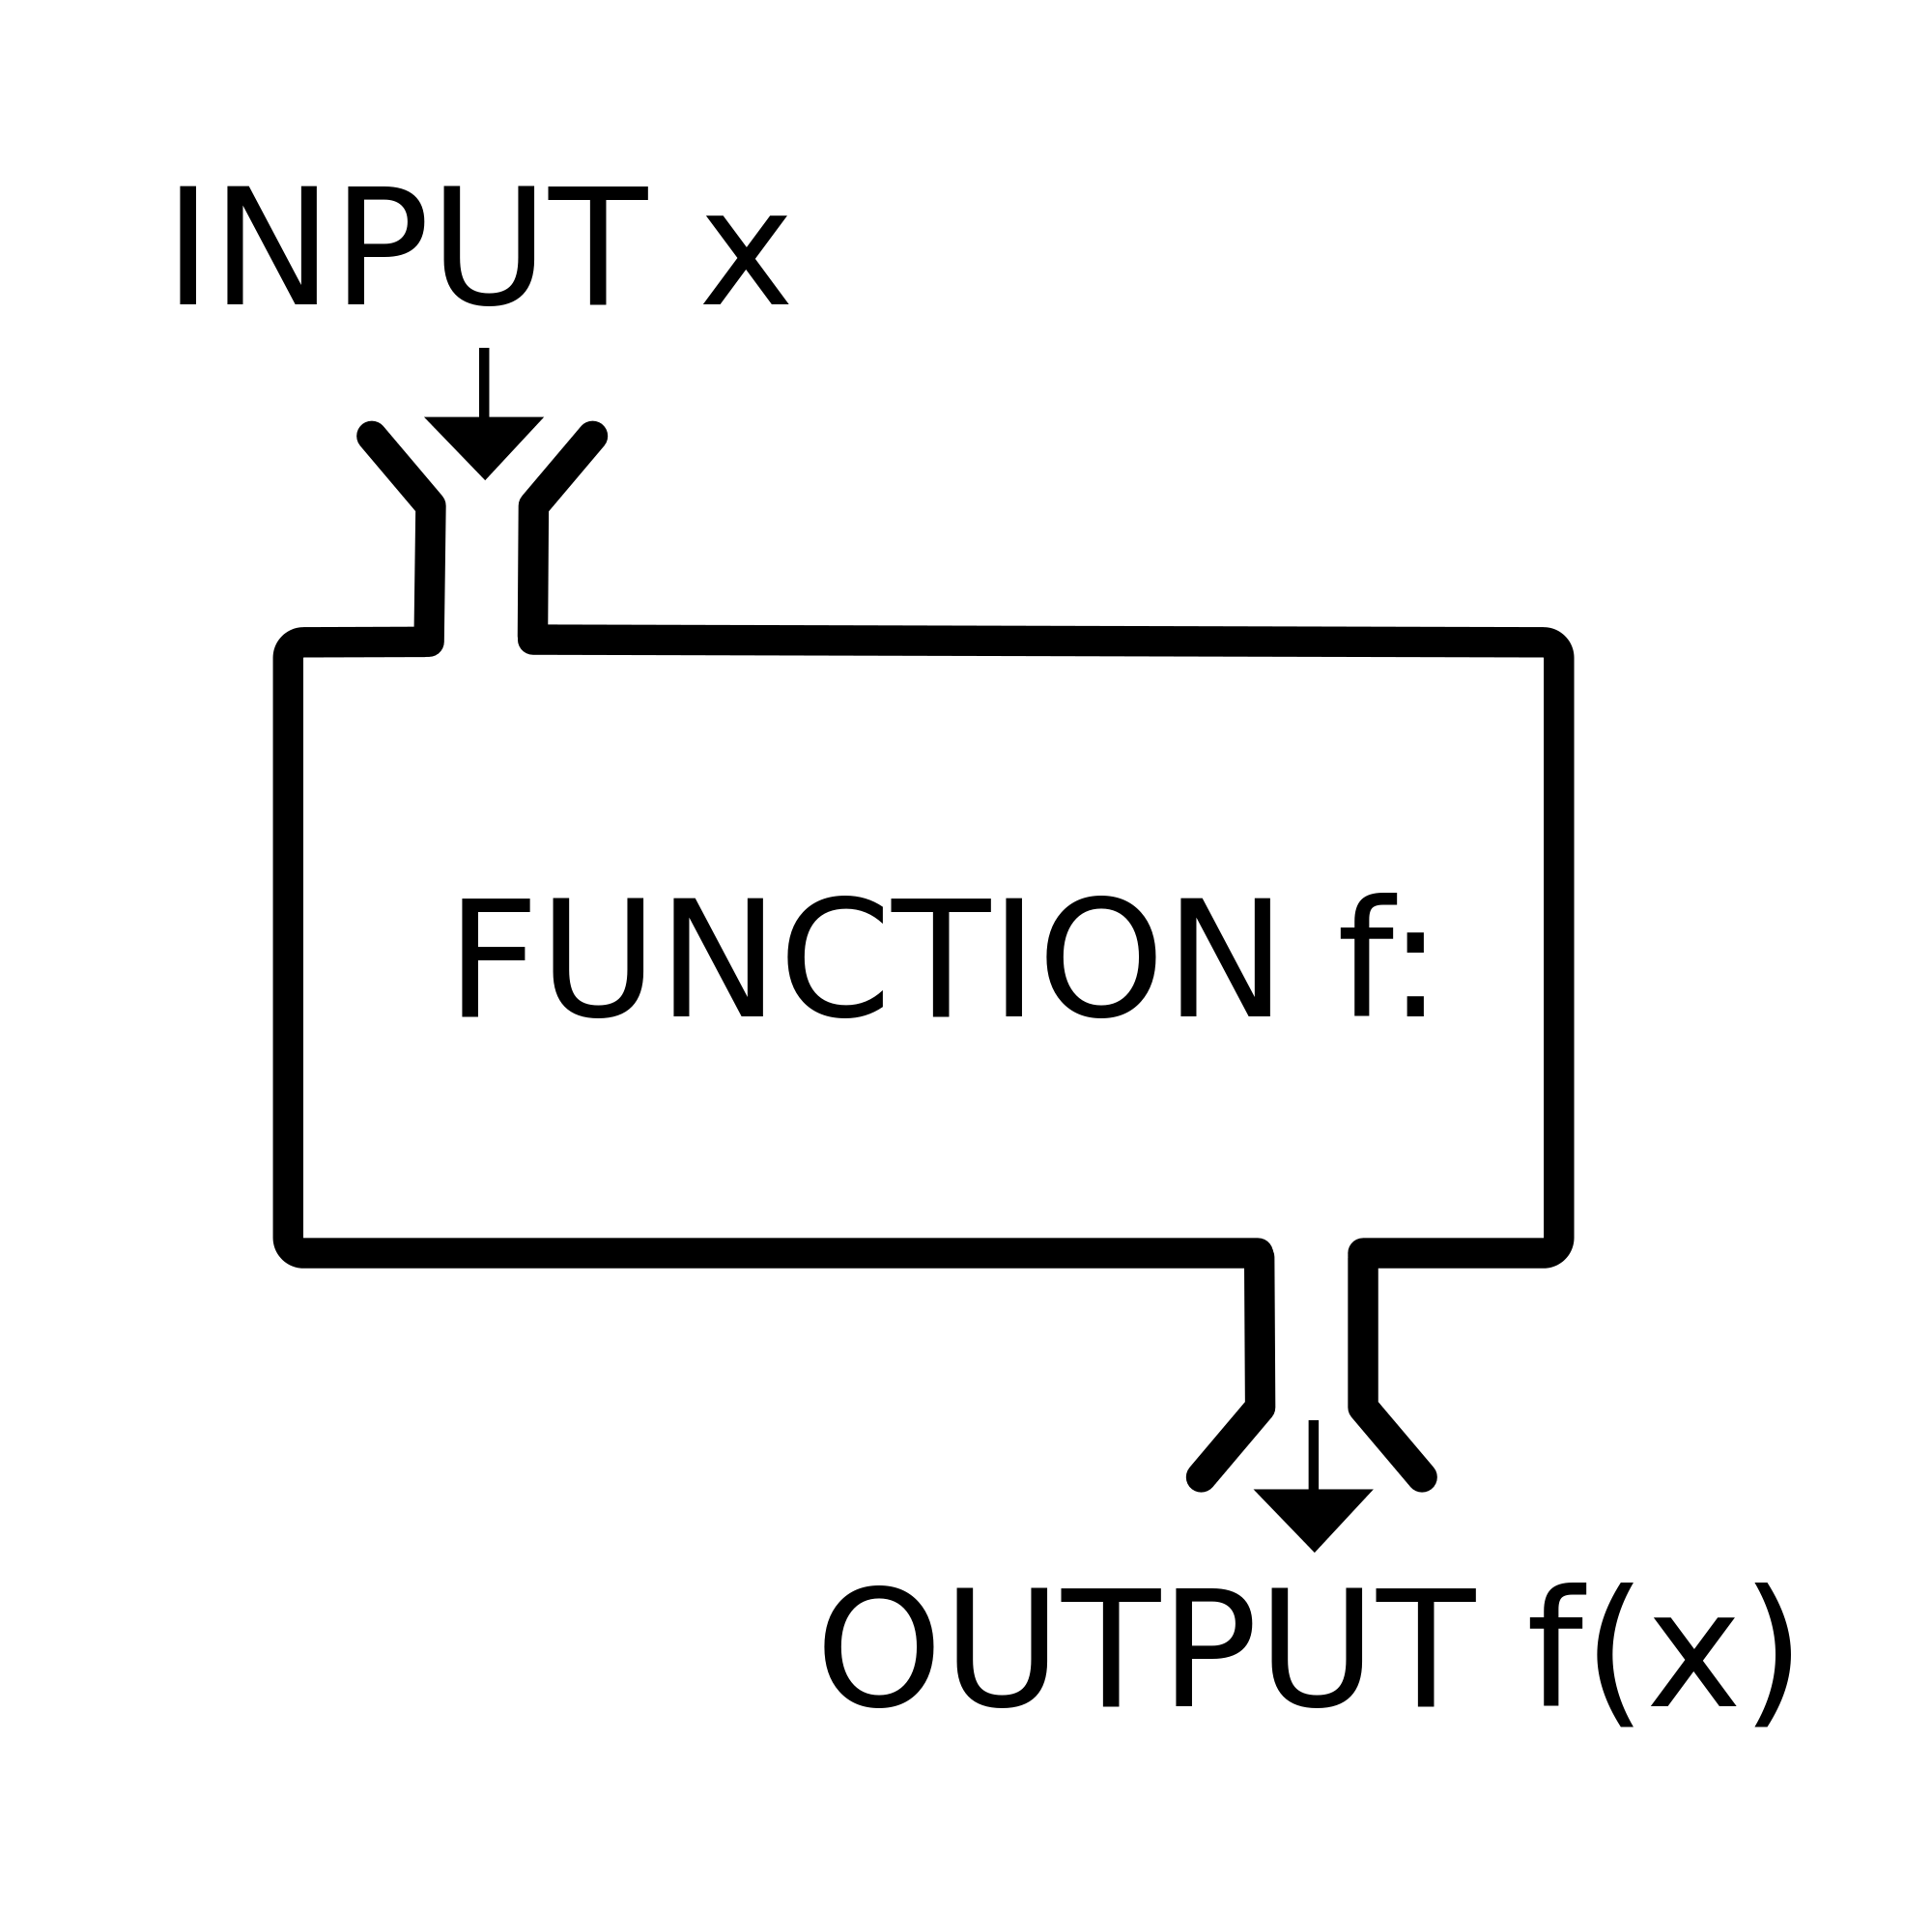
\includegraphics[width=.9\textwidth]{function}
		\end{figure}
\end{frame}
\begin{frame}{$f(x)=x^{2}$}
	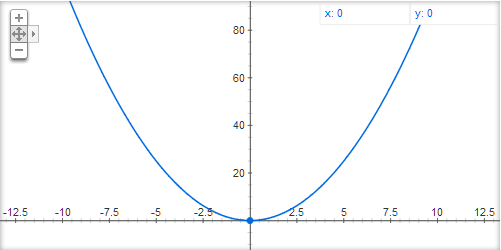
\includegraphics[width=1\textwidth]{xsq}
\end{frame}

\begin{frame}{Using Functions}
	\begin{center}
	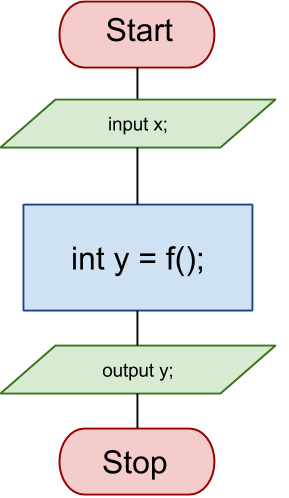
\includegraphics[width=.4\textwidth]{fsq}
	\end{center}
\end{frame}

\begin{frame}{Using Functions}
	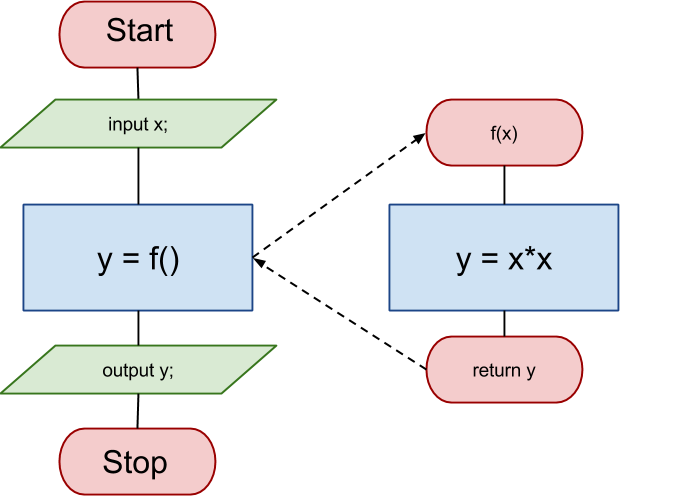
\includegraphics[width=1\textwidth]{fsq_function}
\end{frame}

\begin{frame}[fragile]{Implementing f(x)}
	\begin{center}
	 
	\begin{minted}{c++}
	//prototype
	int f(int x);

	//implementation
	int f(int x){
	   int y = x*x;
	   return y;
	}   
	\end{minted}
	\end{center}
	\begin{center}
		\begin{itemize}
			\item function and return \textbf{must} have same type
			\item parameters can be of various types
		\end{itemize}
	\end{center}
\end{frame}

\begin{frame}[fragile]{Using f(x)}
	\begin{columns}
	 \begin{column}{.49\textwidth}
	\begin{minted}{c++}
	#include <iostream>
	using namespace std;
		
	//function prototype
	int f(int x);

	int main(){
	   int x;
	   cin>>x;
	   int z = f(x);
	   cout<<"f(2)="<<z<<endl;
	   return 0;
	}
	\end{minted}
	\end{column}
	\pause

	\begin{column}{.49\textwidth}
		\begin{minted}{c++}
		//function for computing x^2
		int f(int x){
		    int y = x*x;
		    return y;
		}   
	\end{minted}
	\end{column}
	\end{columns}
\end{frame}

\begin{frame}{practice}
	\begin{itemize}
		\item Write a function named check() that has three parameters. The first parameter should accept an integer number, and the second and third parameters should accept a double-precision number. The function body should display the values of
data passed to the function.
		\item Write a function named rightTriangle() that accepts the lengths of two sides of a right triangle as the arguments a and b. The function should determine and return the hypotenuse, c, of the triangle.
	\end{itemize}
\end{frame}

\begin{frame}[fragile]{Default Args}
	\begin{center}
	\begin{minted}{c++}
	//prototype
	int f(int x=0);

	//implementation
	int f(int x=0){
	   int y = x*x;
	   return y;
	}   
	\end{minted}
	\end{center}
	\begin{center}
	\begin{itemize}
		\item function can have unlimited number of parameters
		\item function can have unlimited number of default args
		\item defaults must come after regular parameters
	\end{itemize}
	\end{center}
\end{frame}

\begin{frame}[fragile]{Default Args: using f(x)}
	\begin{columns}
	 \begin{column}{.49\textwidth}
	\begin{minted}{c++}
	#include <iostream>
	using namespace std;
		
	//function prototype
	int f(int x=0);

	int main(){
	   cout<<"f(0)="<<f()<<endl;
	   return 0;
	}
	\end{minted}
	\end{column}
	\pause
	\begin{column}{.49\textwidth}
		\begin{minted}{c++}
		//function for computing x^2
		int f(int x=0){
		    int y = x*x;
		    return y;
		}   
	\end{minted}
	\end{column}
	\end{columns}
\end{frame}

\begin{frame}{practice}
	\begin{itemize}
		\item modify check() so that the last value defaults to 42
		\item modify rightTriangle() so that if a side isn't intered, it's set as 0
	\end{itemize}
\end{frame}

\begin{frame}[fragile]{Overloading}

	\begin{columns}
	\begin{column}{.49\textwidth}
	\begin{minted}{c++}
	//prototypes
	int f(int x);
	double f(double x);
	
	//implementation
	int f(int x){
	   int y = x*x;
	   return y;
	}
   
	double f(double x){
	   double y = x*x;
	   return y;
	}   
	\end{minted}
	\end{column}
	\begin{column}{.49\textwidth}
	\begin{itemize}
		\item can overload based on parameter type
		\item can also overload based on parameter count
	\end{itemize}
	\end{column}
	\end{columns}
\end{frame}


\begin{frame}[fragile]{Overloading: using f(x)}
	\begin{columns}
	 \begin{column}{.49\textwidth}
	\begin{minted}{c++}
	#include <iostream>
	using namespace std;
		
	//function prototype
	int f(int x);
	double f(double x);

	int main(){
	   int z = f(2);
	   cout<<"f(2)="<<z<<endl;
	   double x = f(2.5);
	   cout<<"f(2)="<<x<<endl;
	   return 0;
	}
	\end{minted}
	\end{column}
	\pause
	\begin{column}{.49\textwidth}
	\begin{minted}{c++}
	int f(int x){
	   int y = x*x;
	   return y;
	}
   
	double f(double x){
	   double y = x*x;
	   return y;
	}
	
	\end{minted}
	\end{column}
	\end{columns}
\end{frame}

\begin{frame}{practice}
	\begin{itemize}
		\item overload check to accept all ints
		\item overload rightTriangle() to accept doubles
	\end{itemize}
\end{frame}

\begin{frame}[fragile]{Pass by reference: f(x)}
	\begin{center}
	 
	\begin{minted}{c++}
	//prototype
	int f(int x, int &y);

	//implementation
	int f(int x, int &y){
	   y = x*x;
	}   
	\end{minted}
	\end{center}
	\begin{center}
		\begin{itemize}
			\item function and return \textbf{must} have same type
			\item parameters can be of various types
		\end{itemize}
	\end{center}
\end{frame}

\begin{frame}[fragile]{Using f(x)}
	\begin{columns}
	 \begin{column}{.49\textwidth}
	\begin{minted}{c++}
	#include <iostream>
	using namespace std;
		
	//function prototype
	int f(int x, int &y);

	int main(){
	   int x, y;
	   cin>>x;
	   f(x, y);
	   cout<<"f(2)="<<y<<endl;
	   return 0;
	}
	\end{minted}
	\end{column}
	\pause
	\begin{column}{.49\textwidth}
		\begin{minted}{c++}
		//function for computing x^2
		int f(int x, int &y){
		   y = x*x;
		}   
		\end{minted}
	\end{column}
	\end{columns}
\end{frame}

\begin{frame}{practice}
	\begin{itemize}
		\item implement the function addn that adds some value n to an input parameter x. The user can set n, but it defaults to 0.
		\item write a function to sort 3 values and return the sorted values
	\end{itemize}
\end{frame}


\begin{frame}{Variable Scope}
	\begin{itemize}
		\item local scope
		\begin{itemize}
			\item only seen by function it's definied in
			\item name can be reused in other functions
		\end{itemize}
		\item global scope
		\begin{itemize}
			\item entire program can see the variable
			\item defined outside main
			\item bad practice-don't use unless required
		\end{itemize}
	\end{itemize}
\end{frame}

\begin{frame}[fragile]{Variable storage allocation}
	\begin{minted}{c++}
		auto int var1;
		static int var2;
		extern int var3;
	\end{minted}
	\begin{description}
		\item[auto (default)] storage allocated on execution
		\item[static] storage allocated on compilation
		\item[extern] storage can be seen by other files
	\end{description}
\end{frame}

\end{document}

